In the first part of this work, we present a neuro-symbolic architecture that learns grounded manipulation programs via visual-linguistic reasoning for instruction understanding over a given scene, to achieve a desired goal. Unlike previous work, we do not assume any sub-goal supervision, and demonstrate how our model can be trained end-to-end. We also make our model interpretable, with the ability to visualise any intermediate state before actual execution. Our experiments show strong generalization to novel scenes and instructions compared to a neural-only baseline.

In the next part, we present a discrepancy-aware neuro-symbolic approach for plan recovery from failures. Unlike existing approaches, we do not require hand-annotated data of failures, rather we make use of self-supervision to train our recovery model. Our approach makes use of object-centric representation of the state in the form a dense scene-graph. We train neural modules to learn the transition function based on data gathered from an existing neuro-symbolic planner. Additionally, we train neural discriminators, trained via the help of other states encountered during execution as negatives, to help us distinguish the representations of the simulated state (desired) from the failure states. Once a failure is detected, a recovery plan is constructed to join back the originally constructed plan at an appropriate point. We present discrepancy-aware heuristics to speed up forward search, and an anytime recovery approach which searches for the best plan within a given budget. Experiments show strong performance compared to baselines, and generalization to larger scenes, longer plans, and greater errors. 

\section{Limitations}

\begin{enumerate}
    \item All experiments have been performed on a Pybullet simulator. Real-robot experiments are necessary to validate our approach, and identify practical real-world challenges which cannot be observed in deterministic simulations.
    
    \item False positives in error detection lead to unnecessary re-tries and recovery plans involving corrrectly placed objects. This can even keep happening in a loop. See figure ~\ref{fig:fp} for an example.

    \item Current object matching approach does not scale well with larger scenes. Object tracking algorithms may perform better in real-time

    \item We currently assume that only a restricted predicate set can denote preconditions for an action. More powerful GNN-based approaches directly applied on the scene-graph may be suited for complex actions.

    \item Due to a single point of view and lack of object tracking, we cannot distinguish between an occluded object and an object which has fallen off the table. In the former case, the situation may still be recoverable, but we mark it as unrecoverable.

    \item An object kept behind another object can be confused with an object kept on top due to issues with 2D bounding box representation. 
    
    \item Our representation has no explicit notion of orientation of objects. The model may not detect a strange orientation as erroneous if the discriminator considers visual features similar. See figure ~\ref{fig:orient} for an example.
\end{enumerate}

\begin{figure}
    \centering
    \begin{subfigure}{.3\textwidth}
        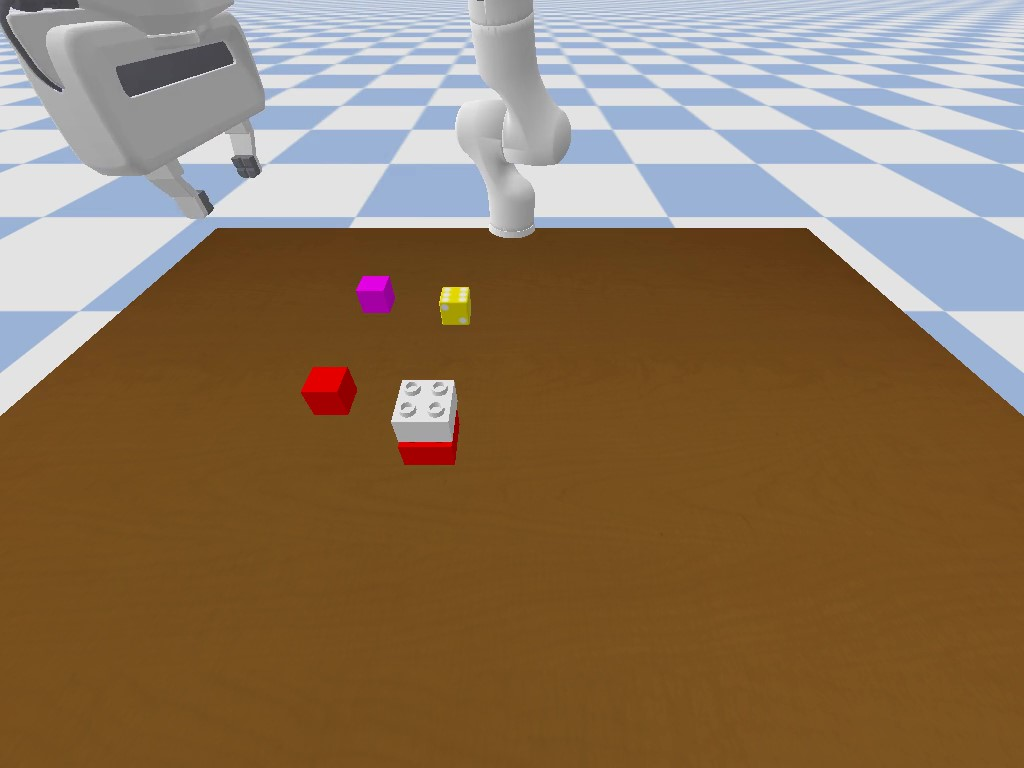
\includegraphics[width=\textwidth]{assets/fp-1.jpg}
    \end{subfigure}
    \hspace{0.3cm}
    \begin{subfigure}{.3\textwidth}
        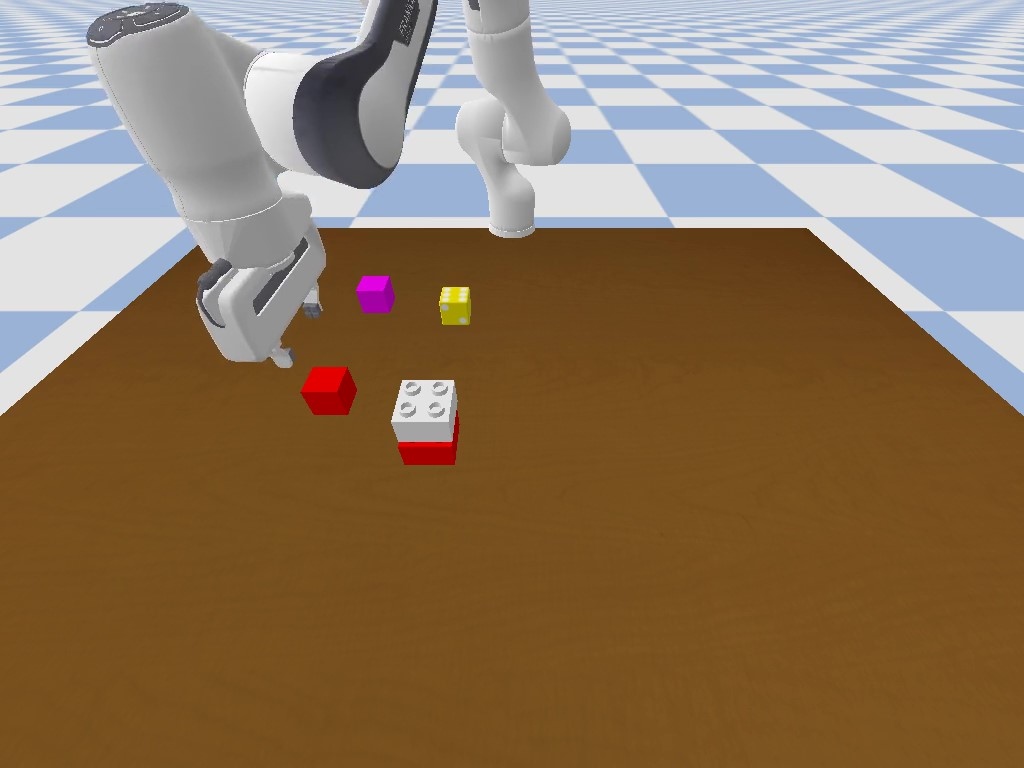
\includegraphics[width=\textwidth]{assets/fp-2.jpg}
    \end{subfigure}
    
    \caption{False positives in error detection. Even though the left state is error free, the model detects a discrepancy in the red block, and picks and places it at its same position.}
    \label{fig:fp}
\end{figure}

\begin{figure}
    \centering
    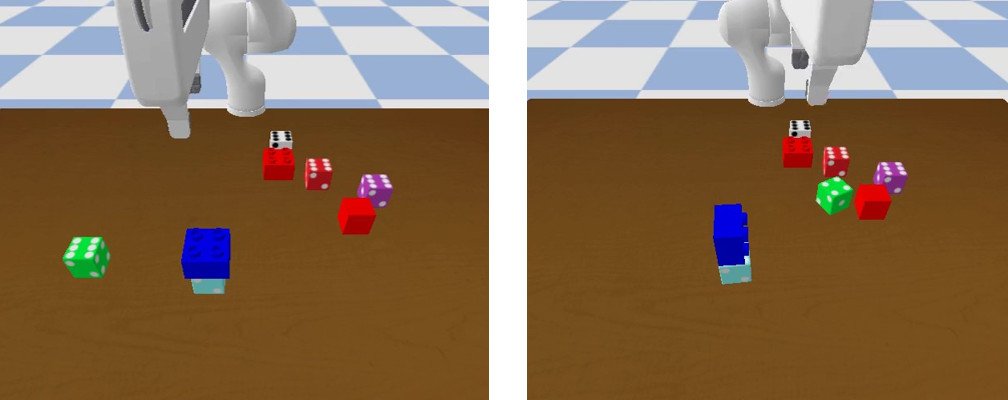
\includegraphics[width=0.7\textwidth]{assets/orient.png}
    \caption{Our representation has no explicit notion of object orientation. The left figure denotes the desired state. The right figure is classified as an error-free state.}
    \label{fig:orient}
\end{figure}

\section{Future work}

\begin{enumerate}
    \item Performing experiments on a real-robot environment with a similar table top setting and a Franka Emika manipulator to confirm our findings, and identify more practical challenges.
    \item Integration of the error-recovery framework with the earlier robot manipulation model for end-to-end training of various modules.
    \item Moving to 3D state representations to solve issues with perception and 2-D representation.
\end{enumerate}

